\chapter{How to Analyse and Represent Quantitative Soundscape Data}\label{ch:circumplex}


Published as: \textbf{Mitchell, A.}, Aletta, F., \& Kang, J. (2022). How to analyse and represent quantitative soundscape data. \emph{JASA Express Letters, 2}(13):037201.

\section*{Context}
The content of this chapter was originally published as \citet{Mitchell2022How}.

\section{Abstract}
This study first examines the methods presented in ISO 12913 for analysing and representing soundscape perception by applying them to a large existing database of soundscape assessments. The key issue identified is the inability of the standard methods to summarise the soundscape of locations and groups. The presented solution inherently considers the variety of responses within a group and provides an open-source visualisation tool to facilitate a nuanced approach to soundscape assessment and design. Several demonstrations of the soundscape distribution of urban spaces are presented, along with proposals for how this approach can be used and developed.

\section{Introduction}
Methods for collecting data on how people experience acoustic environments have been at the forefront of the debate in soundscape studies for the past 20 years. While the soundscape research field as we understand it today dates back to the late 1960s with the pioneering work of authors like M. Southworth \citep{Southworth1969sonic}, R.M. Schafer \citep{SoundscapeOursonicSchafer}, and H. Westerkamp \citep{Westerkamp2002Linking}, the theme of data collection methods for soundscape assessment emerged more prominently only recently \citep{Kang2016Ten}. There is a general consensus in the research community that standardised tools to gather and report individual responses on the perception of urban acoustic environments are indeed desirable, to provide comparable datasets and soundscape characterisations across different locations, times, and samples of people, as well as allowing for replicability studies and offering inputs for modelling algorithms in soundscape prediction and design tasks. These were among the main drivers for the establishment of a Working Group at the \gls{iso} back in 2008, which was named "Perceptual assessment of soundscape quality" (ISO/TC 43/SC1/WG 54) that has so far published three documents within the ISO 12913 series on soundscape. Part 1 (ISO 12913-1:s014) is a full standard and provides a general framework and definitions of soundscape concepts \citep{ISO12913Part1}, while Part 2 (ISO/TS 12913-2:2018) and Part 3 (ISO/TS 12913-3:2019) are technical specifications and offer guidance on how data should be collected and analysed, accordingly \citep{ISO12913Part2,ISO12913Part3} (Part 4, on soundscape design interventions, is currently under development by the working group, also registered as a technical specifications document). Specifically, Part 3 presents the proposed methods for analysing and representing the data collected by the soundscape surveys. Since the development of these standards, the focus has shifted from understanding individual perception to characterising the collective perception of increasingly large groups.

In a recent editorial paper on Soundscape Assessment, Axelsson and colleagues observe that it is important to critically discuss current theories and models in soundscape studies and to examine their effectiveness, while also looking at how to integrate different methods and perspectives for the discipline to make further advancements \citep{Axelsson2019Editorial}. This work was mainly aimed at addressing the issue of meaningful comparability and representation of soundscape assessments. Part 2 of the ISO 12913 standard itself does not provide ultimate answers: the technical specifications recommend multiple methods, as consensus around a single protocol could not be reached. This diversity of methodological approaches should be interpreted as a fact that soundscape theory is still under development and, for this reason, the standardisation work should probably take a step back and focus on developing a reference method for comparability among soundscape studies, rather than a single protocol for soundscape data collection. Some attempts have indeed already been made in literature for the different methods proposed in the ISO/TS 12913-2:2018 \citep{Aletta2019Exploring, jo2020soundscape}. 

This study thus aims to review the consequences of these methods for larger datasets and provide concrete examples for how soundscapes should be represented. In particular, we aim to strengthen the practices for characterising the soundscape of a location, as a collective perception by the users of the location. We also demonstrate how the progress of these tools from their initial scope (measuring and discussing the individual perception of a soundwalk participant) have not kept up with recent advances and requirements for larger-scale soundscape datasets. We question whether there are some issues related to the data collection instruments and data analysis methods as recommended, and examine the results of the model framework and mathematical transformations laid out in the ISO technical specifications in order to provide guidance on the interpretation of the soundscape circumplex. 

To examine these tools and the questions raised, we apply them to an existing large scale, real-world dataset of soundscape assessments collected according to the ISO methods. Finally, we propose a more holistic and advanced method of representing soundscapes as a probabilistic distribution of perceptions within the circumplex and provide a toolbox for others to use.

\section{The current ISO 12913 framework}
\label{sec:current}
Although different methods are proposed for data collection in ISO12913 Part 2 \citep{ISO12913Part2}, in the context of this study we focus on the questionnaire-based soundscape assessment (Method A), because it is underpinned by a theoretical relationship among the items of the questionnaire that compose it. The core of this questionnaire is the 8 perceptual attributes (PA) originally derived in \citet{Axelsson2010principal}: pleasant, vibrant (or exciting), eventful, chaotic, annoying, monotonous, uneventful, and calm. In the questionnaire procedure, these PAs are assessed independently of each other, however they are conceptually considered to form a two-dimensional circumplex with \textit{Pleasantness} and \textit{Eventfulness} on the x- and y-axis, respectively, where all regions of the space are equally likely to accommodate a given soundscape assessment \citep{Aletta2016Soundscape}. In \citet{Axelsson2010principal}, a third primary dimension, \textit{Familiarity} was also found, however this only accounted for 8\% of the variance and is typically disregarded as part of the standard circumplex. As will be made clear throughout, the circumplex model has several aspects which make it useful for representing the soundscape perception of a space as a whole.

\subsection{Coordinate transformation into the two primary dimensions}
To facilitate the analysis of the PA responses, the Likert scale responses are coded from 1 (Strongly disagree) to 5 (Strongly agree) as ordinal variables. In order to reduce the 8 PA values into a pair of coordinates which can be plotted on the Pleasant-Eventful axes, Part 3 of ISO 12913 \citep{ISO12913Part3} provides a trigonometric transformation, based on the $45\degree$-relationship between the diagonal axes and the pleasant and eventful axes. This transformation projects the coded values from the individual PAs down onto the primary Pleasantness and Eventfulness dimensions, then adds them together to form a single coordinate pair. In theory, this coordinate pair then encapsulates information from all 8 PA dimensions onto a more easily understandable and analysable two dimensions. The ISO coordinates are thus calculated by:
\begin{equation}
  \begin{split}
    \label{eqn:pleasant}
    ISO Pleasant = [(pleasant - annoying) + \cos 45\degree * (calm - chaotic) \\ + \cos 45\degree * (vibrant - monotonous)] * 1/(4+\sqrt{32)}
  \end{split}
\end{equation}

\begin{equation}
  \begin{split}
    \label{eqn:eventful}
    ISO Eventful = [(eventful - uneventful) + \cos 45\degree * (chaotic - calm) \\ + \cos 45\degree * (vibrant - monotonous)] * 1/(4+\sqrt{32)}
  \end{split}
\end{equation}
where the PAs are arranged around the circumplex as shown in \cref{fig:radar}. The $\cos 45\degree$ term operates to project the diagonal terms down onto the x and y axes, and the $1 \slash (4 + \sqrt{32})$ scales the resulting coordinates to the range (-1, 1). The result of this transformation is demonstrated in \cref{fig:radar}. This treatment of the 8 PAs makes several assumptions and inferences about the relationships between the dimensions. As stated in the standard \citep[p. 5]{ISO12913Part3}:

\begin{quote}
  According to the two-dimensional model, vibrant soundscapes are both pleasant and eventful, chaotic soundscapes are both eventful and unpleasant, monotonous soundscapes are both unpleasant and uneventful, and finally calm soundscapes are both uneventful and pleasant.
\end{quote}

\begin{figure}
  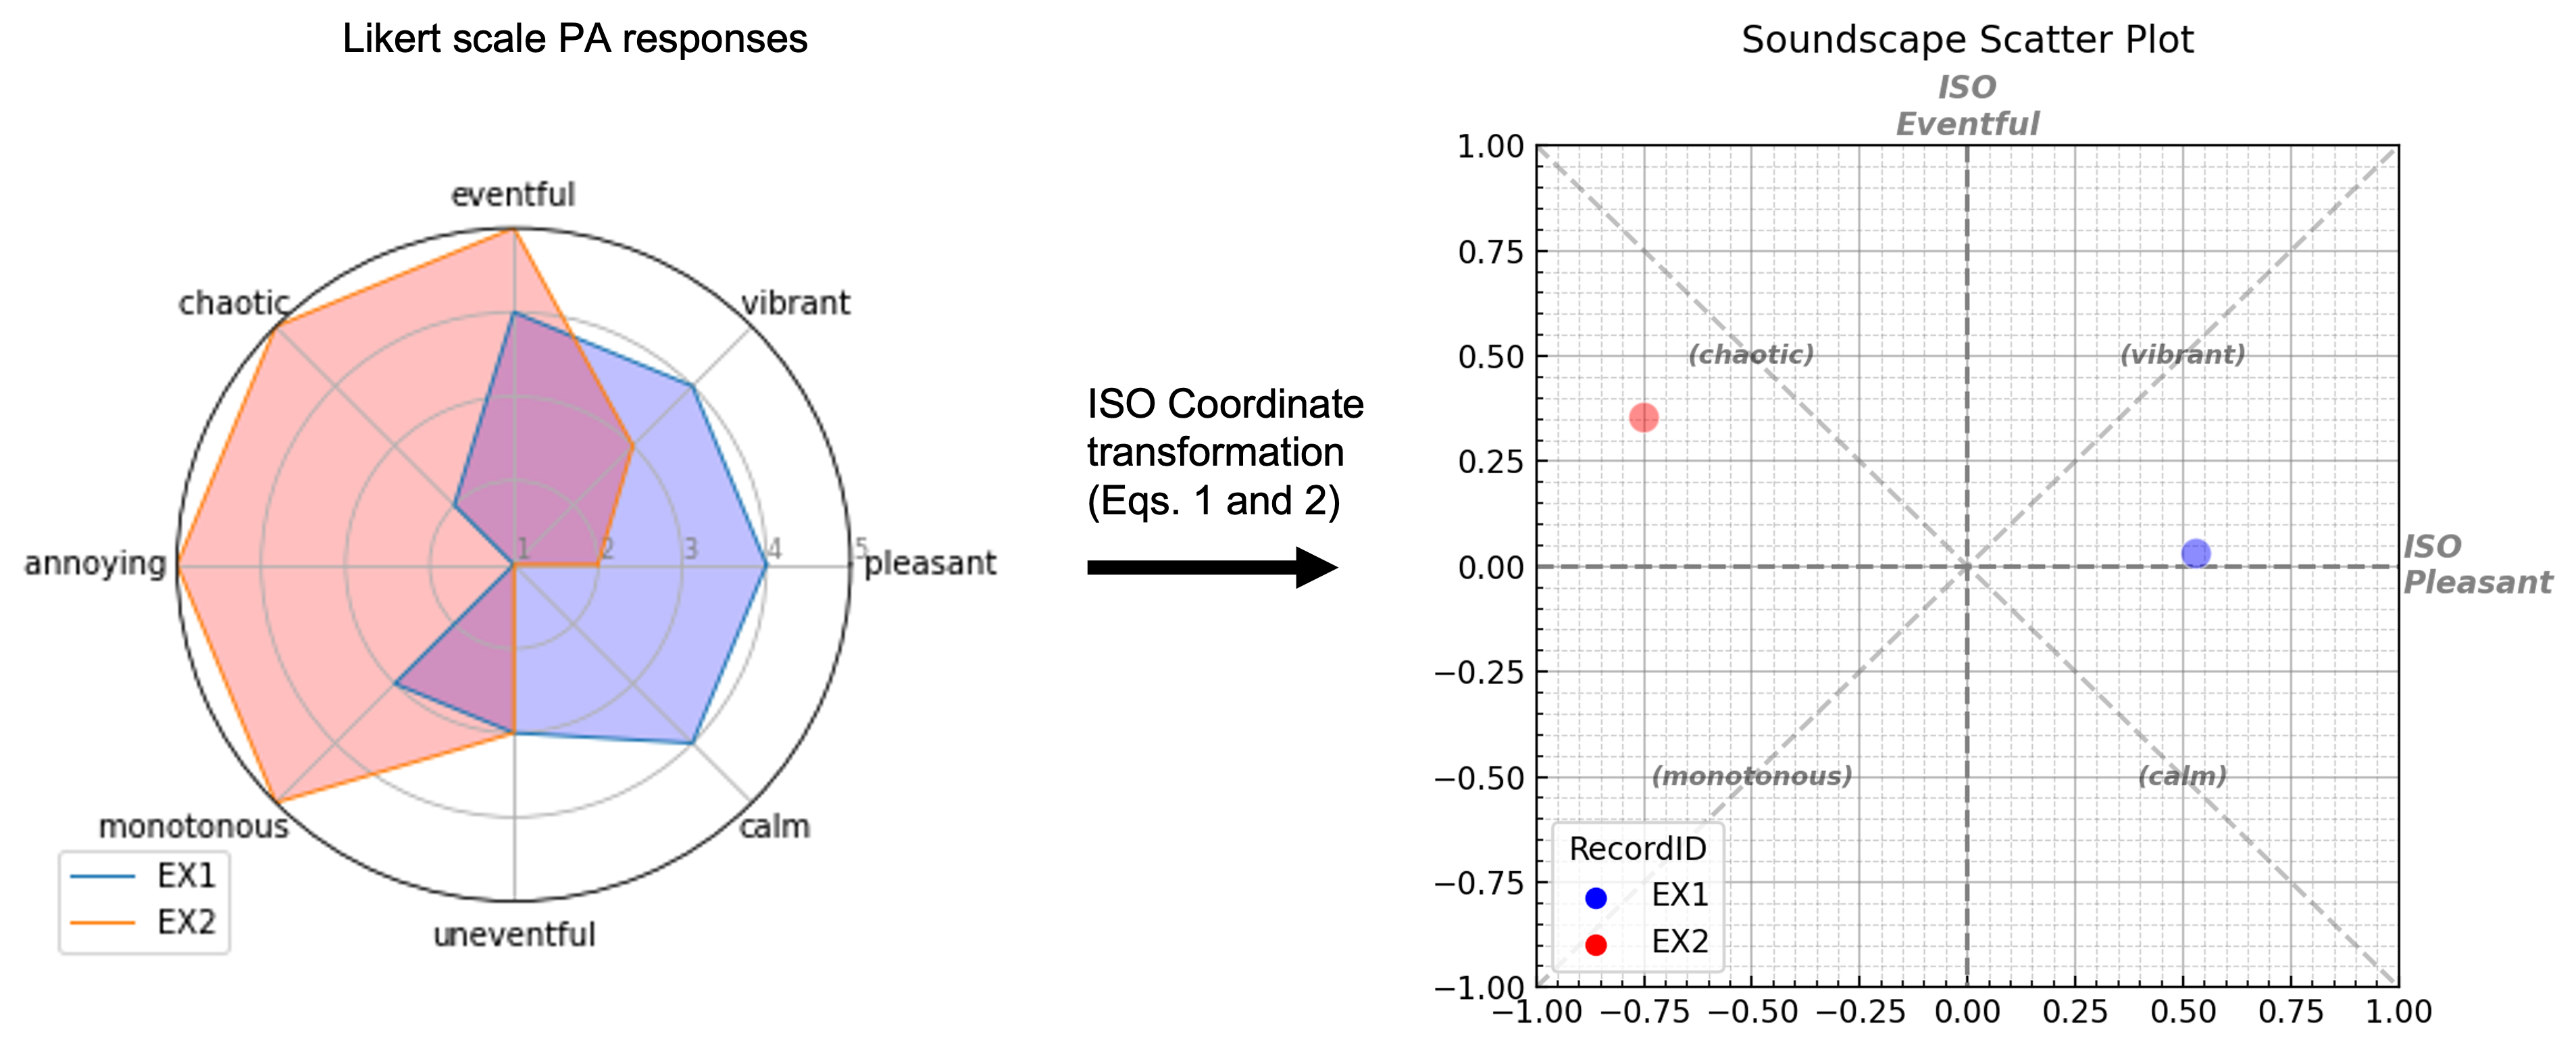
\includegraphics[width=\textwidth]{Figures/jasa-el_Figure1.png}
  \caption{Example of representations of two soundscape assessments. Left: Radar plot of two example perceptual attribute (PA) ratings on the Likert scales (1 to 5). Right: Scatter plot of the same assessments on the soundscape circumplex, transformed according to ISO 12913 Part 3.
    \label{fig:radar}
  }
\end{figure}

\subsection{Summarising the soundscape assessment of a location}
While the assessment methods available are able to record the soundscape perception of a single individual, and that person's perception is valid for themselves, it is not appropriate to then state that it is representative of the collective perception of that soundscape. In order to characterise the soundscape of a particular space or time, perceptual responses from multiple people must be collected and subsequently summarised or aggregated to describe the general soundscape of the location. The ISO guidelines stipulate a minimum of 20 participants for a soundwalk, with these broken up into sessions of no more than 5 participants at a time. Part 3 then provides the recommended methods for analysing this data.

Annex A.2 of ISO 12913 Part 3 provides the statistical measures to be used on the raw PA responses. The recommended measure of central tendency is the median, while the recommended measure of dispersion is the range. These are chosen as the data is ordinal by nature, however as will be demonstrated later, they have significant limitations. Although it is unclear, the implied intention is then that the median value of each PA is fed into \cref{eqn:pleasant,eqn:eventful} presented above to calculate the ISOPleasant and ISOEventful values, which can then be plotted in a two-dimensional scatter plot.

\subsection{Limitations of the ISO}
How these methods should be applied to represent the soundscape of a location has not been adequately discussed in previous literature, nor sufficiently in Part 3 of ISO 1293 itself. Indeed, in Section A.3, the technical specifications document state that \citep[p. 5]{ISO12913Part3}:

\begin{quote}
  Results can be reported in a two-dimensional scatter plot with coordinates for the two dimensions ‘pleasantness’ and ‘eventfulness’. The coordinates for ‘pleasantness’ are plotted on the X-axis, and the coordinates for ‘eventfulness’ on the Y-axis. Every data point in the scatter plot represents one investigated site.
\end{quote}

However, it is not made clear whether this single point on the circumplex can be considered to be a realistic representation of the average perception of the acoustic environment. Effectively, there is no representation of dispersion in the soundscape assessment, nor a recommended use of the range that was calculated as part of the analysis recommend in Section A.2 of Part 3 of the ISO 12913. Absent a suggestion from the ISO 12913 for how the range should be used, we therefore apply this analysis to an existing real-world soundscape dataset to determine whether it provides a useful measure of dispersion. Here we use the data contained in the International Soundscape Database (ISD) \citep{Mitchell2021International}, which includes 1,300+ individual responses collected across 13 locations in London and Venice, according to the SSID Protocol, which is based on the ISO methods explored in this paper \citep{Mitchell2020Soundscape}.

For any large enough sample for a site, the range will always be from 1 to 5, the maximum and minimum available Likert-scale values. We would expect that collecting more data would result in more information or better precision, however the range will always increase as the sample size increases. As an example, within the ISD data, of the 8 PAs collected at 13 locations (for a total of 104 scales), 88\% have a range from 1 to 5 and with larger sample sizes at each location, this percentage would only have increased. Using range to analyse the dispersion provides very limited information for comparing the soundscape assessments of different locations, or of a location under different conditions.

Although the range does not appear to be a useful measure of dispersion, the median does provide a useful measure and appropriately functions to describe the central tendency of the  soundscape assessment of the sample. However, by stipulating that the median of each PA should be taken prior to applying the circumplex projection, the ISO procedure only allows for plotting a single scatter point in the circumplex for each location, and does not allow for plotting individual responses on the circumplex. This limits the possibilities for visualising the general trends in individual perception across the soundscape. Finally, no example or recommendation for how the circumplex scatter plot should be presented is given in the standard.

The instruments described in the ISO 12913 Part 2 \citep{ISO12913Part2} were originally designed primarily for the context of individual or small group assessments. In these scenarios, the focus is on assessing the particular soundscape perception of the person in question. Recent advances in the soundscape approach since the development of the standards have shifted some focus from individual soundscapes to characterising the overall soundscape of public spaces \citep{Mitchell2020Soundscape} and to making comparisons between different groups of people \citep{Jeon2018cross}. In this context, a consideration of the natural variation in people's perception and the variation over time of a soundscape must be a core feature of how the soundscape is discussed. Reducing a public space which may have between tens and tens of thousands of people moving through it in a single day down to the mean (or median, or any other single metric) soundscape assessment often dismisses the reality of the space. Likewise, this overall soundscape of a public space cannot be determined through a ten person soundwalk, as there is no guarantee that the sample of people engaged in the soundwalk are representative of the users of the space (in fact it is very likely they would not be).


\section{The Way Forward: Probabilistic Soundscape Representation}
Given the identified issues with the recommended methods for statistical analysis and their shortcomings in representing the variety in perception of the soundscape in a space, how then should we discuss or present the results of these soundscape assessments? Ideally the method will: 1) take advantage of the circumplex coordinates and their ability to be displayed on a scatter plot and treated as continuous variables, 2) scale from a dataset of twenty responses to thousands of responses, 3) facilitate the comparison of the soundscapes of different locations, conditions, and groups, and 4) encapsulate the nuances and diversity of soundscape perception by representing the distribution of responses.

We therefore present a visualisation in \cref{fig:circ} of the soundscape assessments of several urban spaces included in the ISD \citep{Mitchell2021International} which reflects these goals. The specific locations selected from the ISD are chosen for demonstration only and these methods can be applied to any location. Rather than attempting to represent a single individual's soundscape or of describing a location's soundscape as a single average assessment (as in \citep{Mitchell2021Investigating}), this representation shows the whole range of perception of the users of the space. First, rather than calculating the median response to each PA in the location, then calculating the circumplex coordinates, the coordinates for each individual response are calculated. This results in a vector of ISOPleasant, ISOEventful values which are continuous variables from -1 to +1 and can be analysed statistically by calculating summary statistics (mean, standard deviation, quintiles, etc.) and through the use of regression modelling, which can often be simpler and more familiar than the recommended methods of analysing ordinal data. This also enables each individual's response to be placed within the pleasant-eventful space. All of the responses for a location can then be plotted, giving an overall scatter plot for a location, as demonstrated in (i).

\begin{figure}[!ht]
  \centering
  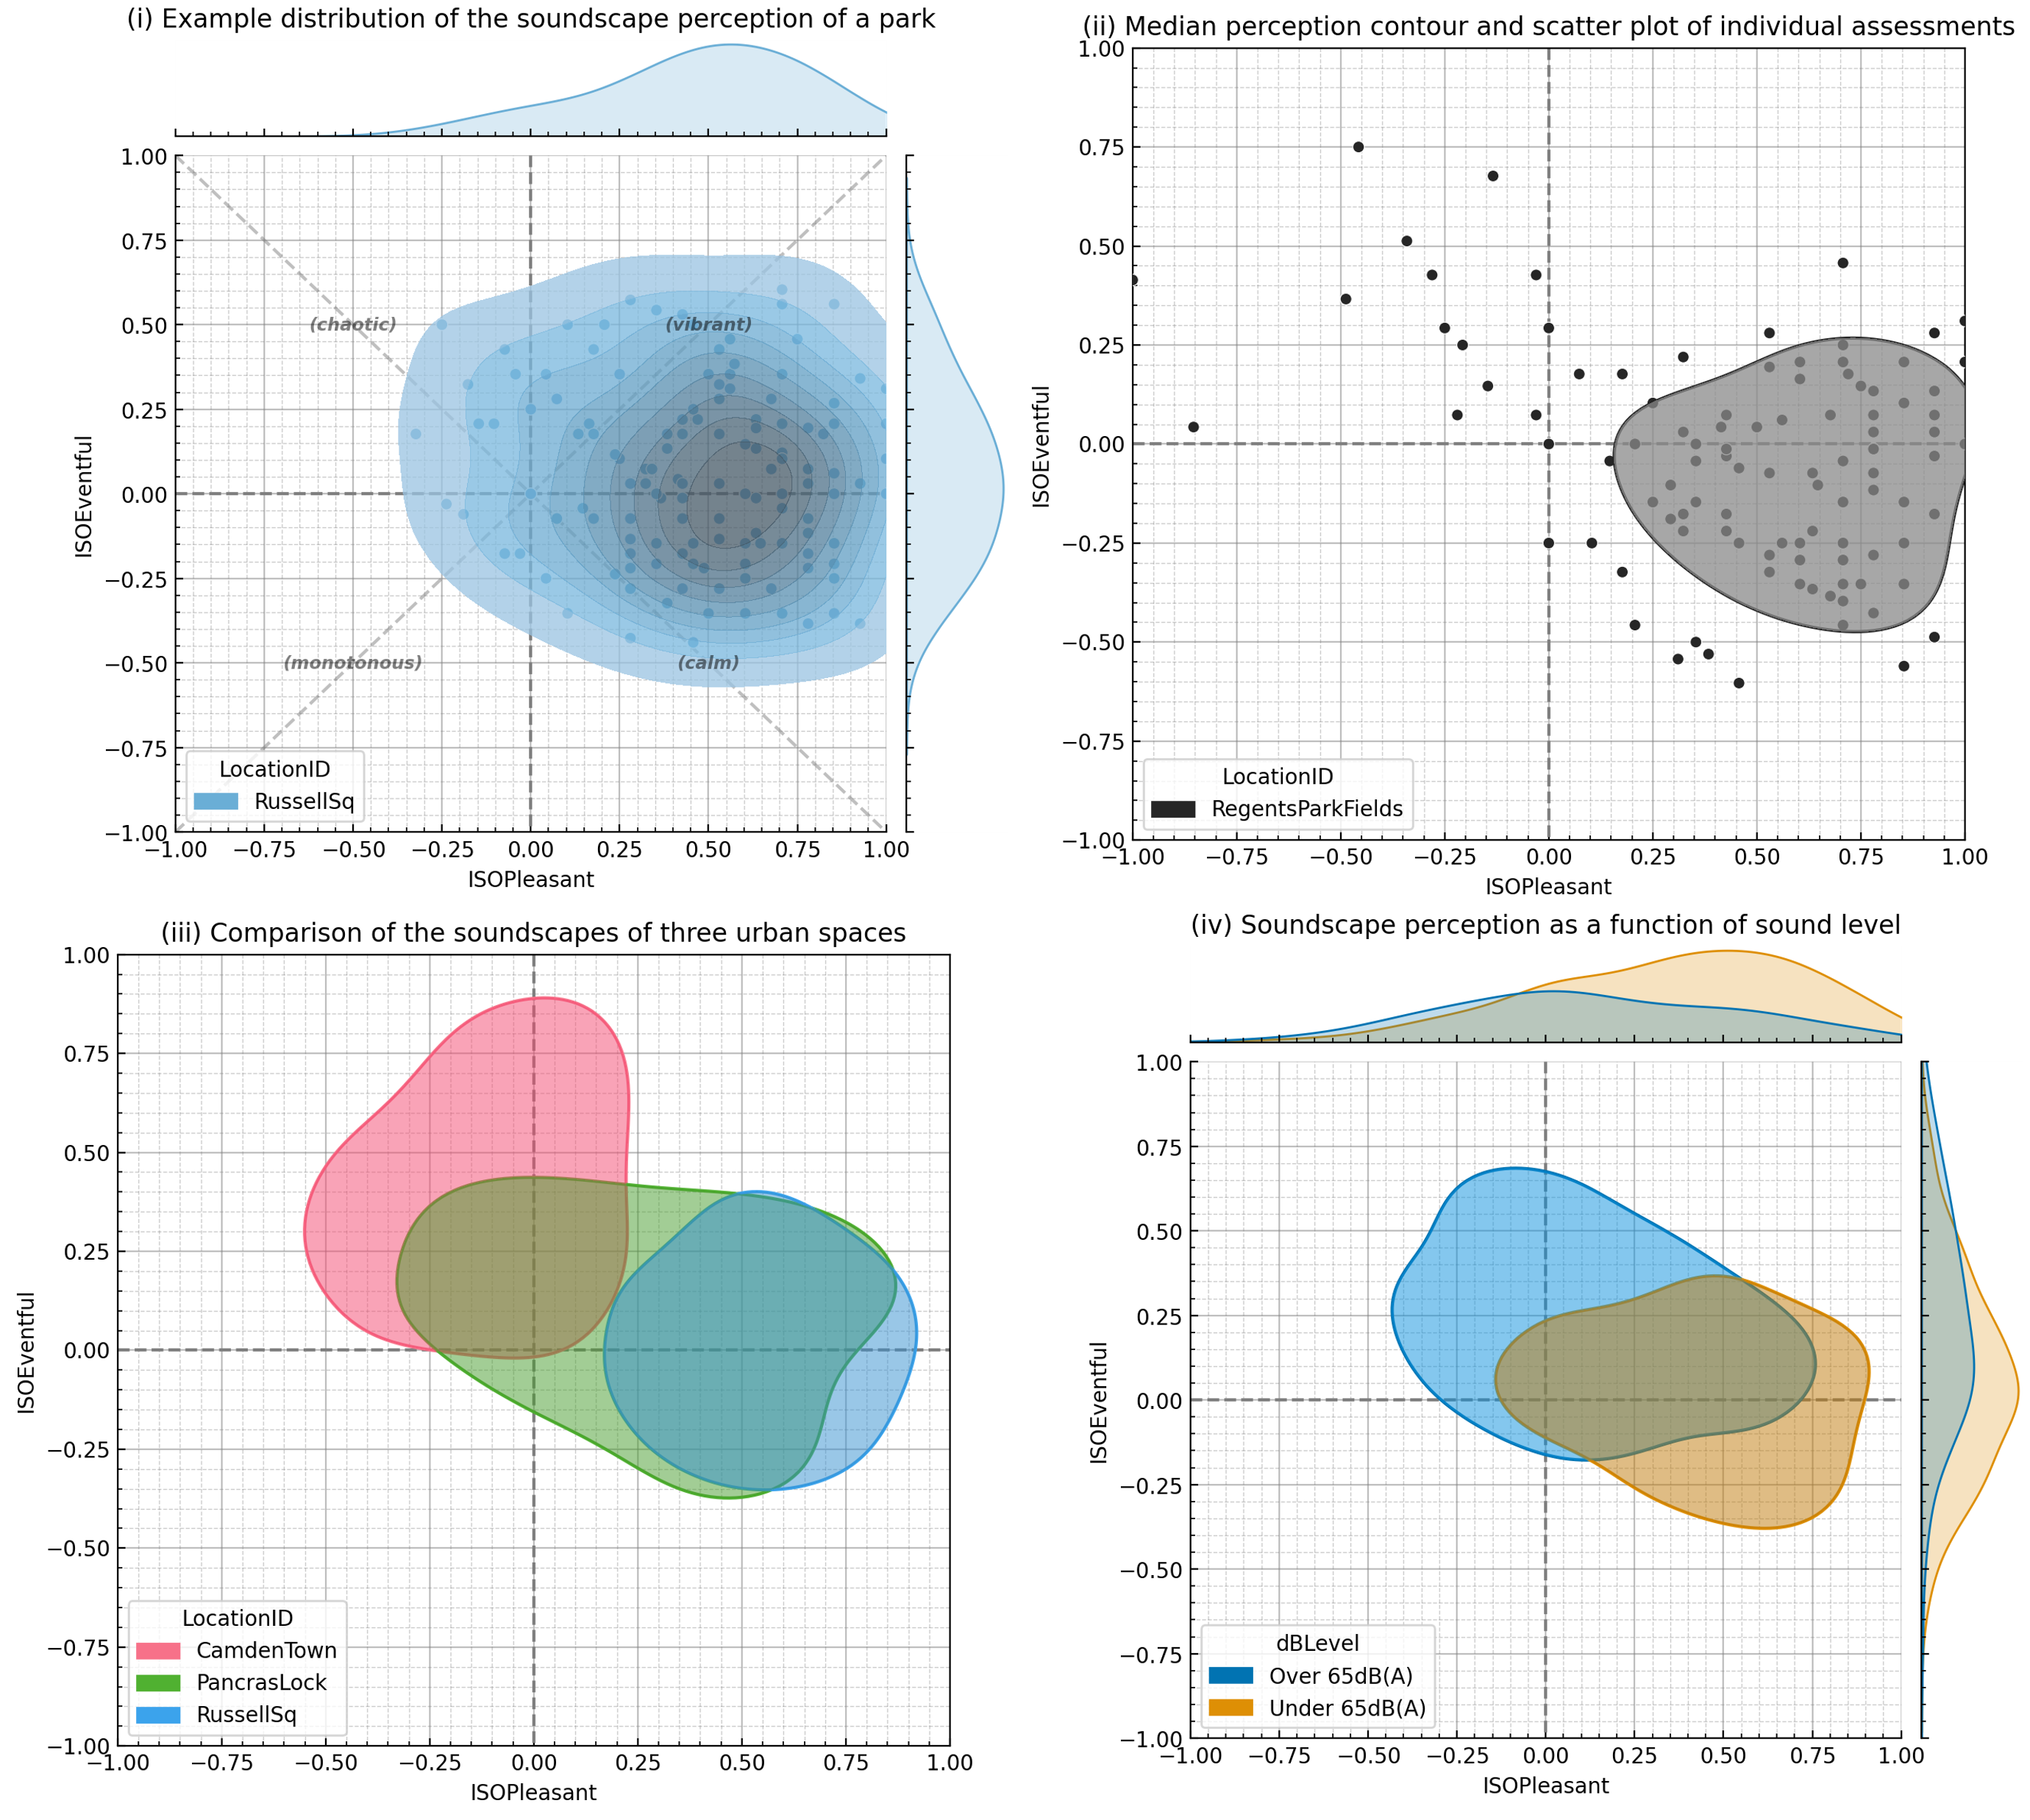
\includegraphics[width=\textwidth]{Figures/jasa-el_Figure2.png}
  \caption{\linespread{1}\selectfont{} A demonstration of some use cases of representing soundscape perception as probabilistic distributions. Data is drawn from the International Soundscape Database (ISD) and is used for demonstration only. (i) Demonstrates a high-level of detail for presenting the bivariate distribution of soundscape perception in a park (Russell Square in London). (ii) Simplified view of the distribution using the \nth{50} percentile contour. The assessments impacted by a series of helicopter fly-overs are made obvious in the chaotic quadrant. (iii) A comparison of three popular public spaces in London. Their overlapping regions can reveal when and how their soundscapes may be similar. (iv) A comparison across the full ISD for soundscape perception at $<65 dB L_{Aeq}$ and $> 65 dBA$. The introduction of other acoustic, environmental, and contextual data can reveal new and complex relationships with the soundscape perception. \label{fig:circ}}
\end{figure}

Once these individual responses are plotted, we then overlay a heatmap of the bivariate distribution (with isodensity curves for each decile) and marginal distribution plots. In this way, three primary characteristics of the soundscape perception can be seen:

\begin{enumerate}
  \item The distribution across both pleasantness and eventfulness, including the central tendency, the dispersion, and any skewness in the response;
  \item The general shape of the soundscape within the space - in this case Russell Sq is almost entirely in the pleasant half, but is split relatively evenly across the eventfulness space, meaning while it is perceived as generally pleasant, it is not strongly calm or vibrant;
  \item The degree of agreement about the soundscape perception among the sample - there appears to be a relatively high agreement about the character of Russell Sq, as demonstrated by the compactness of the distribution, but this is not the case for every location.
\end{enumerate}

Fig (i) includes several in-depth visualisations of the distribution of soundscape assessments, however the detail included can make further analysis difficult. In particular, a decile heatmap is so visually busy that, in our experience, it is not possible to plot more than one soundscape distribution at a time without the figure becoming overly busy. It also can make it difficult to truly grasp point 2, the general shape of the soundscape. To facilitate this, the soundscape can be represented by its \nth{50} percentile contour, as demonstrated in Fig (ii) where the shaded portion contains 50\% of the responses. This simplified view of the distribution presents several advantages, as is demonstrated in Figs. (iii and iv) and takes inspiration from the recommendation in the ISO standard to use the median as a summary statistic. In our testing, the \nth{50} percentile contour has proved useful, clear, and compact, however this should not be taken as the definitive correct percentile cutoff. Further work will need to be done to validate the precise presentation.

When visualised this way, it is possible to identify outliers and responses which are the result of anomalous sound events. For instance if, during a survey session at a calm park, a fleet of helicopters flies overhead, driving the participants to respond that the soundscape is highly chaotic, we would see a group of scatter points in the chaotic quadrant which appear obviously outside the general pattern of responses. Often, these responses would be entirely discarded as outliers or the surveys and soundwalks would be halted entirely -- ignoring what is in fact a significant impact on that location, its soundscape, and how useful it may be for the community. Alternatively, they would be naively included within the statistical analysis, significantly impacting the central tendency and dispersion metrics (i.e. median and range) without consideration for the context. This is the situation shown in Fig (ii) where it is obvious that there is strong agreement that Regents Park Fields is highly pleasant and calm, however we can see numerous responses which assessed it as highly chaotic. These responses were taken when a series of military helicopter fly overs drastically changed the sound environment of the space for nearly 20 minutes.

Fig (iii) demonstrates how this simplified \nth{50} percentile contour representation makes it possible to compare the soundscape of several locations in a sophisticated way. The soundscape assessments of three urban spaces, Camden Town, Pancras Lock, and Russell Square, are shown overlaid with each other. We can see that Camden Town, a busy and crowded street corner with high levels of traffic noise and amplified music, is generally perceived as chaotic, but the median contour shape which characterises it also crosses over into the vibrant quadrant. We can also see that, for a part of the sample, Russell Square and Pancras Lock are both perceived as similarly pleasant, however some portion of the responses perceived Pancras Lock as being somewhat chaotic and annoying. This kind of visualisation is able to highlight these similarities between the soundscapes in the locations and identify how they differ. From here, further investigation could lead us to answer what factors led to those people perceiving the location as unpleasant, and what similarities the soundscape of Pancras Lock has with Russell Square that could perhaps be enhanced to increase the proportion of people perceiving it as more pleasant.

In addition to solely analysing the distributions of the perceptual responses themselves, this method can also be combined with other acoustic, environmental, and contextual data. The final example, in Fig (iv) demonstrates how this method can better demonstrate the complex relationships between acoustic features of the sound environment and the soundscape perception. The data in the ISD includes ~30-s-long binaural audio recordings taken while each participant was responding to the soundscape survey, providing an indication of the exact sound environment they were exposed to. For Fig (iv) the entire dataset of 1,338 responses at all 13 locations has been split according to the analysis of these recordings giving a set of less than 65 dB $L_{Aeq}$ and a set of more than 65 dB. The bivariate distribution of these two conditions are then plotted.

By presenting soundscape perception as a bivariate distributional shape on the circumplex, practitioners are obligated to address two key aspects of perception that are too often ignored: the distribution of potential responses and the eventful dimension. The array of potential responses to an environment is a crucial factor in assessing the successful design of a space and represents the reality of perception. There is no single perceptual outcome of an environment; it will always include some randomness inherent in human perception and this should be reflected in how we present soundscape assessments. Similarly, the eventful dimension is crucial to understanding how an environment is perceived and can have important impacts on the health and well-being of the users. Recent evidence also suggests that there is a more direct relationship between acoustic characteristics and the perception of eventfulness, while pleasantness is more dependent on context \citep{Mitchell2021Investigating}. Studies which explore the correlations between acoustic features and annoyance (or pleasantness) without considering eventfulness are perhaps missing the most direct effect of the acoustic features.

A library of plotting functions for producing the type of plots presented here has been made available as part of the ISD at \href{https://zenodo.org/record/5705908}{https://zenodo.org/record/5705908}. In addition, an interactive code notebook for this paper is included which provides a tutorial for using this code, working with the ISD data, and recreating the figures of this paper. The figures were created using the seaborn \citep{Waskom2021seaborn} and Matplotlib \citep{Hunter2007Matplotlib} plotting libraries in Python v3.92 \citep{VanRossum2009}.

\section{Making Use of the Soundscape Circumplex}
There are various potential methods for integrating the probabilistic soundscape approach into a design and intervention setting. Representing the soundscape as a shape within the circumplex provides flexibility in setting design goals for a space. Not all spaces can or should have the same soundscape and soundscapes should be treated as dynamic, not static; identifying and creating an appropriate soundscape for the particular use case of a space is crucial to guiding its design. Proper forward-looking design of a soundscape would involve defining the desired shape and distribution of perceptions in the space. This can be achieved by drawing the desired shape in the circumplex and testing interventions which will bring the existing soundscape closer to the desired perception. A soundscape may need to be perceived as vibrant during the day and calm for some portion of the evening, meaning the desired shape should primarily sit within the vibrant quadrant but have some overlap into calm. This also enables designers to recognise the limitations of their environment and acknowledge that it is not always possible to transform a highly chaotic soundscape into a calm one. In these cases, instead the focus should be placed on shifting the distribution to some degree in a positive direction. The most sophisticated method of setting design goals is therefore to identify the desired shape which represents the variety of desired outcomes, and focus on designs and interventions which are most successful in matching the predicted outcome with that goal.

Although the visualisations shown in \cref{fig:circ} are a powerful tool for viewing, analysing, and discussing the multi-dimensional aspects of soundscape perception, there are certainly cases where simpler metrics are needed to aid discussion and to set design goals. Taking inspiration from noise annoyance \citep{ISO15666}, we propose a move toward discussing the "percent of people likely to perceive" a soundscape as pleasant, vibrant, etc. when it is necessary to use numerical descriptions. In this way, a numerical design goal could also be set as e.g. `the soundscape should be likely to be perceived as pleasant by at least 75\% of users' or the result of an intervention presented as e.g. `the likelihood of the soundscape being perceived as calm increased from 30\% to 55\%'. These numbers can be drawn from either actual surveys or from the results of predictive models.

Finally, although acknowledging the distribution of responses is crucial, it is sometimes necessary to summarise locations down to a single point to compare many different locations and to easily investigate how the soundscape assessment has generally changed over time. For this purpose, the mean of the ISOPleasant and ISOEventful values across all respondents is calculated to result in a single coordinate point per location. This clearly mirrors the original intent of the coordinate transformation presented in the ISO, but by applying the transformation first to each individual assessment then calculating the mean value, it maintains a direct link to the distributions shown in \cref{fig:circ}. An example plot using the mean response of each location to compare many locations and to demonstrate change in soundscape perception can be found in Figure 5 of \citet{Mitchell2021Investigating}. The key to all of these analysis methods, whether they be the distributional plots shown in \cref{fig:circ}, the numerical summaries, or the use of other standard statistical analyses is treating the soundscape of the space or group as a collective perception as expressed by a vector of individual circumplex coordinates.

\subsection{Incorporating appropriateness}

The discussion thus far has focussed on the two primary dimensions of soundscape perception - pleasantness and eventfulness. Our next goal is to somehow account for the third primary component identified by \citet{Axelsson2010principal} - Familiarity, sometimes also referred to as Appropriateness. In a later paper, \citet{Axelsson2015How} addresses critiques of the \gls{ssqp} for its focus on perceptual attributes and its use of a Good-Bad scale, without considering the appropriateness of the soundscape. %TODO Return here


\subsection{Limitations of the circumplex and quantitative analysis}
The method presented here is a solution for representing the soundscape of a space, which requires considering the perception of many people, but it is important to note that this is only one (very important) goal of the soundscape approach. Psychological and sociological investigations of people's relationship to their sound environment and the interactions between social contexts and individual perception are a crucial aspect of the field for which this approach would likely not be sufficient \citep{Bild2018Public}. Open-response questions, structured interviews, and mixed-methods studies can provide additional insight into how people experience their environment and should be considered alongside or preceding this focus on how a space is likely to be perceived on a larger scale.

These other approaches are not in opposition to the methods proposed here, but instead further expand our view. The circumplex is a limited view of soundscape perception (this is made obvious by the fact that it excludes the third component, \emph{familiarity}, identified in \citet{Axelsson2010principal}) but it is an exceptionally rich tool for dealing with the two primary aspects of soundscape perception which can readily expand the much more limited view provided by existing noise and annoyance assessment tools. Aspects of the psychological and sociological emphasis can also be integrated into a circumplex-focused approach, as demonstrated in \citet{Erfanian2021Psychological}, where personal factors such as age, gender, and psychological well-being were analysed in terms of how they mediated the ISOPleasant and ISOEventful outcomes.

It should also be noted that the particular PA descriptors used in ISO 12913 are intended for outdoor environments and should not be directly applied to indoor spaces. However, a proposed set of descriptors for some indoor environments has been derived which further confirms the validity of the circumplex relationships \citep{Torresin2020Indoor}. The methods proposed here should be directly applicable to indoor spaces by using the comfort/content descriptors as well as to any other translations of soundscape descriptors into other languages \citep{Aletta2020Soundscape} as long as the dimensional relationships of the circumplex are maintained.


\section{Conclusions}
Soundscape studies have been steadily growing as a research field over the past three decades. Their relevance for the planning and design of urban spaces is now generally acknowledged by both the academic and practitioners' communities. Yet, for their contribution in shaping better environments to be meaningful, it is necessary to agree on common methodological approaches and techniques to analyse and present standardised soundscape data. Therefore, the general goal of this work is to consider some of the questions that may still have been left unanswered by the ISO 12913 series when it comes to optimal ways to analyse and represent soundscape data coming from the ISO standardised protocols. As a result, we propose a method for presenting the results of standardised
assessments as a distribution of soundscape perception within the circumplex space. This method provides an opportunity to conduct a nuanced discussion of soundscape perception which considers the variety of individual responses. The tools for generating these circumplex visualisation is made openly available as well. This shift is part of a move towards a more holistic approach to urban noise and to integrating the soundscape approach into urban design and regulations.

%%%%%%%%%%%%%%%%%%%%%%%%%%%%%%%%%%%%%%%%%%%%%%%%%%%%%%%%%%%%%%%%%%%%%%%%%

\draft{======= Random bits to incorporate somewhere =======}
\subsubsection{Sound perception as a chaotic system}

Human perception of sound is a chaotic system. Given small changes in a large number of input conditions, a wide range of outcomes are possible \cit{some chaos theory thing}. The same person, exposed to the same environment, could have very different responses to it depending on their state of mind, the route they took to get to the space, what they ate for breakfast, or even just some inherent randomness in their psychological response. This is further amplified by the innumerable differences between people which it will never be possible to fully capture. This is all the more true when discussing in situ perception, outside the controlled conditions of a laboratory.

However, the wide array of previous literature demonstrates that, when taken as a statistical group, conclusions can be made about the probable soundscape perception and its various causal factors.

\begin{quote}
    It means that in many situations, all we can say about a system's dynamics is of a statistical nature. -Gert van der Hejden
\end{quote}

\section{Interpreting the Soundscape Circumplex}
%Move this paragraph to the interpretation of the circumplex section.
The circumplex model of soundscape, as originally defined by \citet{Axelsson2010principal}, is commonly understood to be a two-dimensional space (its main orthogonal components being annoying-pleasant and uneventful-eventful) where all regions of the space are equally likely to accommodate a given soundscape assessment \citep{Aletta2016Soundscape}. For instance, in theory, an extremely vibrant soundscape (e.g., with a score of 1) should be as likely to occur as an extremely annoying one, as well as one neutral on all dimensions (e.g., with a score of 0). However, a recent work by Lionello et al. \citep{Lionello2021Introducing} incidentally highlighted a possible issue with the process for representing soundscape assessments with the current ISO protocols. More specifically, when considering big numbers, soundscape assessments seem to have a bivariate normal distribution around the origin of the circumplex model. This would imply that not the whole space of the model is equally accessible to any given soundscape. Studies in the field show that data collection campaigns rarely return extreme values for soundscape dimensions \citep{Mancini2021Soundwalk} and so far the general interpretation has been that some soundscapes (e.g., extremely monotonous) may simply be difficult to find and detect with people in urban contexts \citep{Sun2019Classification}. 

\subsection{Application \& Simulations}
In order to investigate the shape of the circumplex coordinate space generated by this transformation, a dataset of 3 million randomly simulated PA responses was generated. For each of the 8 PAs, an integer value from 1 to 5 is randomly generated from a uniform distribution, meaning each of the five responses is equally likely. These simulated data are specifically not intended to include any information about correlations between the various PAs when actually answered by respondents (see \citep{Lionello2021Introducing} for more on this discussion), instead the PA responses are completely uncorrelated as they each have their own random distribution. Therefore, the simulated dataset represents a theoretical uniform coverage of the 8 dimensional PA space.

We then apply the ISO transformations given in \cref{eqn:pleasant,eqn:eventful}, resulting in 3 million coordinate pairs with a range of (-1, 1) in the x and y axes. A heatmap of the resulting two-dimensional circumplex space is shown in \cref{fig:isoheatmap}, along with histograms of the individual dimension distributions. These distributions then represent the theoretical available circumplex space generated by the ISO transformation on uniform survey responses.

\begin{figure}
  %TODO: Insert heatmap figure, with histograms/distribution plots of individual axes
  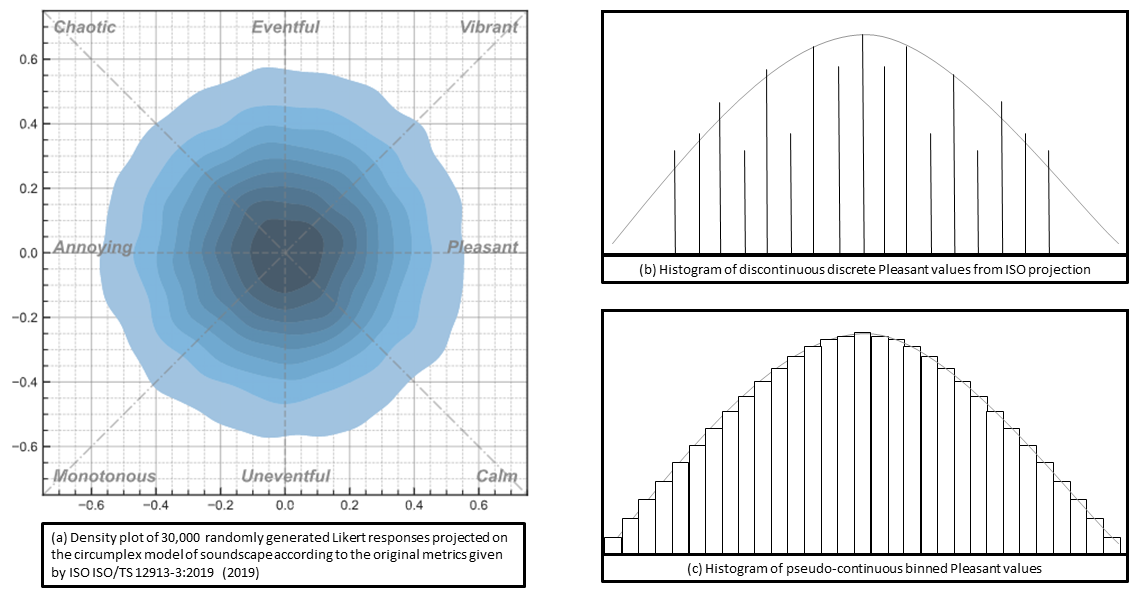
\includegraphics[width=\textwidth]{figures/Combined_sim_hist_mockup.png}
  \caption{Mockup placeholder simulation heatmap plot from Lionello 2020 and discrete vs binned transformation values. For new one, need to include distribution histograms along each axis.%
    \label{fig:isoheatmap}
  }
\end{figure}

Two important observations can be made about the shape of the resulting two-dimensional distribution. The first is that the shape of the available space is a circle. It should be noted that, despite what the term 'circumplex' may indicate, the perceptual dimensions are not necessarily intended to circumscribe a circle. The second is that, in each dimension, the responses are normally distributed, centered around zero. These points will be discussed in detail below.

\subsection{Circular space discussion}
%TODO: fill in circular discussion.
Visualisations of the circumplex model in soundscape literature tend to present it as circumscribing a circle (see Figure 1 in \citep{Axelsson2010principal} and Figure 3 in \citep{Torresin2020Indoor}), and this shape is further emphasised by the initial figure in \citet{Russell1980circumplex}'s original formulation of the concept. However, it should be emphatically noted that all of these presentations are in fact artefacts of the analysis methods which generated them, not some sort of revealed pattern in the component attributes which make up the circumplex. In \citet{Russell1980circumplex}, this first figure is generated by asking respondents to place each of the 27 attributes around a circle, according to their perceived spatial relationships - the circle shape was pre-imposed on the study. In both \citet{Axelsson2010principal} and \citet{Torresin2020Indoor}, the figures are generated via Principle Components Analysis (PCA) which, again, presents these results superimposed on a circle. It is perhaps a weakness of these two, otherwise strong and impactful, papers, that they did not recognise this consequence and challenge the circular arrangement.

If we turn back to Russell's original work on the circumplex model of affect, we can see some indications that a circle does not, in fact, describe the spatial relationship of the perceptual attributes. Fig. 4 of \citep{Russell1980circumplex}, which did not pre-impose the circular arrangement in its analysis, instead most closely resembles a square with rounded corners. Continuing from this conception, when Russell presents a graphical method of assessing the two dimensions of affect (pleasure and arousal) \citep{Russell1989Affect}, they use a square grid. This is all to say that, although the term 'circumplex' and the foundational analyses which lead to a soundscape circumplex may lead us to assume it must take the form of a circle, both the framework laid down by Russell and the common treatment of the spatial relationships of the attributes actually describe a square, instead.

This treatment of the 8 PAs makes several assumptions and inferences about the relationships between the dimensions. As stated in the standard \citep[p. 5]{ISO12913Part3}:

\begin{quote}
  According to the two-dimensional model, vibrant soundscapes are both pleasant and eventful, chaotic soundscapes are both eventful and unpleasant, monotonous soundscapes are both unpleasant and uneventful, and finally calm soundscapes are both uneventful and pleasant.
\end{quote}

From this, we would infer that a maximally vibrant soundscape is both maximally pleasant and maximally eventful. However, when the projection transformation is applied it imposes certain limitations on the relationships between the dimensions which do not conform with this assumption. As shown in \cref{fig:radar}, when a soundscape is maximally vibrant (i.e. a diagonal vector distance of 1), the maximum pleasantness value it can have is determined by the $\cos 45\degree$ term, giving a max pleasantness value of $\sim0.7071$. The implication of this is that no soundscape can be both maximally pleasant and maximally eventful at the same time, meaning that these dimensions are not in fact considered as orthogonal, and that a highly vibrant soundscape cannot be considered highly pleasant or highly eventful. Similarly, if a soundscape were to begin at a maximum Eventfulness, with neutral Pleasantness, in order for the soundscape to become more pleasant, it must by definition become less eventful. This is not conceptually correct or borne out in the treatments of previous literature. These same relationships and violations hold true for the other diagonal dimensions, chaotic, calm, and monotonous.

This implication violates both the assumptions made within the formulation of the circumplex model and the way that soundscape practitioners have understood and presented the interpretations of soundscapes within the circumplex space. In cases where the PA dimensions are referred to directly \citep{steele2016evaluation, steele2019soundtracking} and those which have made use of the Part 3 transformation to 2-dimensional coordinates \citep{Mancini2021Soundwalk, Lionello2021Introducing, Manzano2021importance}, \emph{Check Manzano2021importance} the conflation of maximal values on the diagonal axes with maximal values on the primary axes is made, as in the assumptions made by the standard. This is the first of the common understandings of the circumplex which are violated by the trigonometric transformation.

\subsection{Normal distribution discussion}
%TODO: fill in normal discussion

We can also see from the histograms included along the axes of \cref{fig:isoheatmap} that the projection creates a normal distribution in both dimensions. % TODO: edit this phrasing to match the final figure
It is important here to remember that the input to the projection formulas were uniform distributions for each of the 8 PAs, and it is the projection into the two primary dimensions which results in this normal distribution.
From the simulated distributions, we can derive a normal probability density distribution (PDF) for each of the dimensions.

\[   f_X(x) = \frac{x^{-(x-\mu)^2/(2\sigma^2)}}{\sigma \sqrt{2\pi}}\]
% ! TODO: Need to pull the actual standard deviation value.
with a mean $\mu = 0$ and standard deviation $\sigma = 0.3$.

\paragraph*{Realistic max values}
% ! TODO: Andrew update this with the actual values from the calculations!
When looking at the distribution heatmap in \cref{fig:isoheatmap}, it is useful to picture the gradients as representing the available space in the circumplex model. The probability of reaching a given result decreases as we move farther away from the origin. This means, for example, that the probability of getting a pleasantness value between 0.2 and 0.3 is nearly 4 times the probability of getting a value between 0.5 and 0.6. This may not seem important, but the consequence is that, as a result of strictly the projection calculation, neutral values within the soundscape circumplex are much more likely and the space available to compare soundscapes within is truncated.

When we start to think about real-world urban soundscape data collection, where the discussion of the soundscape of a space is not limited to a single person's perception, we need to start thinking in statistical terms. Theoretically, the limits of the projected Pleasantness are (-1, +1), however according to the PDF calculated above less than 10\% of values fall outside the range (-0.5, +0.5).
% Note: Maybe this should be moved to Proposals or Discussion section?
It may be argued that as long as +1 can theoretically be reached, this should be what is considered the maximum value for that dimension. However, in any situation which involves using multiple individual soundscape assessments in order to characterize the overall soundscape of a location, this max will effectively never be reached. According to the large-scale, multi-location data set reported in our previous study, it appears that the effective maximum values for Pleasantness and Eventfulness for the combined assessment of multiple people for a space is in reality approximately (-0.6, +0.6) \citep{Lionello2021Introducing}.

As such, extreme values on each of the perceptual dimensions are less likely to occur than are coordinate values which place the soundscape in the neutral areas of the circumplex space. This means an extremely calm (or chaotic, or vibrant, or pleasant) coordinate is significantly less likely to occur than a neutral coordinate.


\subsection{Non-continuous projected values}
% Very brief presentation of this potential issue
An implicit assumption of the transformation is that the resulting coordinates are now continuous values, which allows linear regression and correlation methods to be used. Indeed, the transformation of the 8-dimensional ordinal Likert scale data to the two-dimensional coordinates creates a higher resolution of intervals, which would appear to be pseudo-continuous. Upon further investigation, the transformation actually results in XX discrete possible values. \cref{fig:isoheatmap}(b) shows a histogram of this raw output from the transformation, demonstrating that these discrete values, while following the general normal distribution discussed above, are not evenly filled - some adjacent values may be much more or less likely than their neighbours. This poses potential issues for further analysis which assumes either continuous or equally-spaced discrete values.


